% Options for packages loaded elsewhere
\PassOptionsToPackage{unicode}{hyperref}
\PassOptionsToPackage{hyphens}{url}
\PassOptionsToPackage{dvipsnames,svgnames,x11names}{xcolor}
\PassOptionsToPackage{space}{xeCJK}
\documentclass[
  a4paper,
  10pt]{article}
\usepackage{xcolor}
\usepackage{amsmath,amssymb}
\setcounter{secnumdepth}{5}
\usepackage{iftex}
\ifPDFTeX
  \usepackage[T1]{fontenc}
  \usepackage[utf8]{inputenc}
  \usepackage{textcomp} % provide euro and other symbols
\else % if luatex or xetex
  \usepackage{unicode-math} % this also loads fontspec
  \defaultfontfeatures{Scale=MatchLowercase}
  \defaultfontfeatures[\rmfamily]{Ligatures=TeX,Scale=1}
\fi
\usepackage{lmodern}
\ifPDFTeX\else
  % xetex/luatex font selection
  \setmainfont[]{Times New Roman}
  \setmonofont[]{Menlo}
  \setmathfont[]{STIX Two Math}
  \ifXeTeX
    \usepackage{xeCJK}
    \setCJKmainfont[]{Songti SC}
  \fi
  \ifLuaTeX
    \usepackage[]{luatexja-fontspec}
    \setmainjfont[]{Songti SC}
  \fi
\fi
% Use upquote if available, for straight quotes in verbatim environments
\IfFileExists{upquote.sty}{\usepackage{upquote}}{}
\IfFileExists{microtype.sty}{% use microtype if available
  \usepackage[]{microtype}
  \UseMicrotypeSet[protrusion]{basicmath} % disable protrusion for tt fonts
}{}
\usepackage{graphicx}
\makeatletter
\newsavebox\pandoc@box
\newcommand*\pandocbounded[1]{% scales image to fit in text height/width
  \sbox\pandoc@box{#1}%
  \Gscale@div\@tempa{\textheight}{\dimexpr\ht\pandoc@box+\dp\pandoc@box\relax}%
  \Gscale@div\@tempb{\linewidth}{\wd\pandoc@box}%
  \ifdim\@tempb\p@<\@tempa\p@\let\@tempa\@tempb\fi% select the smaller of both
  \ifdim\@tempa\p@<\p@\scalebox{\@tempa}{\usebox\pandoc@box}%
  \else\usebox{\pandoc@box}%
  \fi%
}
% Set default figure placement to htbp
\def\fps@figure{htbp}
\makeatother
\setlength{\emergencystretch}{3em} % prevent overfull lines
\providecommand{\tightlist}{%
  \setlength{\itemsep}{0pt}\setlength{\parskip}{0pt}}
\usepackage[a4paper,top=24mm,bottom=25mm,left=23mm,right=23mm,headheight=15pt]{geometry}
\usepackage{amsmath,amssymb,mathtools,bm}
\usepackage{booktabs,longtable,array}
\usepackage{graphicx}
\usepackage{float}
\usepackage{caption}
\usepackage{enumitem}
\usepackage{fancyhdr}
\usepackage{titlesec}
\usepackage{mdframed}
\usepackage{xcolor}
\usepackage{xurl}
\usepackage{hyperref}
\graphicspath{{../../}}

\definecolor{PaperBlue}{HTML}{000000}
\definecolor{PaperRule}{HTML}{B7C6D5}
\definecolor{PaperShade}{HTML}{F4F7FA}
\definecolor{PaperText}{HTML}{000000}

\hypersetup{
  colorlinks=true,
  linkcolor=PaperBlue,
  urlcolor=PaperBlue,
  citecolor=PaperBlue,
  pdfborder={0 0 0}
}

\color{PaperText}
\linespread{1.08}
\setlength{\parindent}{1.5em}
\setlength{\parskip}{0.25em}
\setlength{\emergencystretch}{3em}
\setlist{itemsep=0.2em,topsep=0.45em}
\setcounter{secnumdepth}{3}
\setcounter{tocdepth}{3}

\titleformat{\section}
  {\Large\bfseries\color{PaperBlue}}
  {\thesection}{0.7em}{}
\titleformat{\subsection}
  {\large\bfseries\color{PaperText}}
  {\thesubsection}{0.65em}{}
\titleformat{\subsubsection}
  {\normalsize\bfseries\color{PaperText}}
  {\thesubsubsection}{0.6em}{}
\titlespacing*{\section}{0pt}{2.2ex plus 0.5ex}{0.9ex}
\titlespacing*{\subsection}{0pt}{1.8ex plus 0.4ex}{0.7ex}
\titlespacing*{\subsubsection}{0pt}{1.5ex plus 0.3ex}{0.5ex}

\captionsetup{
  font=small,
  labelfont=bf,
  textfont=it,
  justification=centering,
  skip=6pt
}

\pagestyle{fancy}
\fancyhf{}
\fancyhead[L]{\small\nouppercase{\leftmark}}
\fancyhead[R]{\small Selene's Blog}
\fancyfoot[C]{\small\thepage}
\renewcommand{\headrulewidth}{0.4pt}
\renewcommand{\footrulewidth}{0pt}
\fancypagestyle{plain}{
  \fancyhf{}
  \fancyhead[R]{\small Selene's Blog}
  \fancyfoot[C]{\small\thepage}
  \renewcommand{\headrulewidth}{0.4pt}
}

\renewenvironment{quote}
  {\begin{mdframed}[
      linewidth=0.7pt,
      linecolor=PaperRule,
      backgroundcolor=PaperShade,
      leftline=true,
      rightline=false,
      topline=false,
      bottomline=false,
      innerleftmargin=10pt,
      innerrightmargin=8pt,
      innertopmargin=7pt,
      innerbottommargin=7pt,
      skipabove=8pt,
      skipbelow=10pt
    ]\itshape}
  {\end{mdframed}}

\newenvironment{theorembox}[1]
  {\par\medskip\noindent\textbf{Theorem (#1).}\quad}
  {\par\medskip}

\newenvironment{lemmabox}[1]
  {\par\medskip\noindent\textbf{Lemma #1.}\quad}
  {\par\medskip}

\newenvironment{proofbox}
  {\par\medskip\noindent\textit{Proof.}\quad}
  {\hfill$\square$\par\medskip}

\AtBeginDocument{\allowdisplaybreaks[2]}
\usepackage{bookmark}
\IfFileExists{xurl.sty}{\usepackage{xurl}}{} % add URL line breaks if available
\urlstyle{same}
% fallback for those not using the hyperref driver hyperxmp:
\makeatletter
\@ifundefined{xmpquote}{\newcommand{\xmpquote}[1]{#1}}{}
\makeatother
\hypersetup{
  pdftitle={CS224N \textbar{} Language Models and Recurrent Neural Networks},
  pdfauthor={Selene},
  colorlinks=true,
  linkcolor={black},
  filecolor={Maroon},
  citecolor={Blue},
  urlcolor={black},
  pdfcreator={LaTeX via pandoc}}

\title{CS224N \textbar{} Language Models and Recurrent Neural Networks}
\author{Selene}
\date{August 20, 2026}

\begin{document}
\maketitle

\section{Language Models}\label{language-models}

A language model computes the probability that a sequence of words
appears in a particular order. The probability of a sequence of \(m\)
words, \(\{w_1,\ldots,w_m\}\), is denoted by \(P(w_1,\ldots,w_m)\).
Because the number of words preceding \(w_i\) depends on its position in
the input document, practical models usually do not condition
\(P(w_1,\ldots,w_m)\) on the entire history. Instead, they approximate
it by conditioning only on the previous \(n-1\) words:

\[
P(w_1,\ldots,w_m)
=\prod_{i=1}^{m}P(w_i\mid w_1,\ldots,w_{i-1})
\approx\prod_{i=1}^{m}P(w_i\mid w_{i-n+1},\ldots,w_{i-1}).
\]

\subsection{n-gram Language Models}\label{n-gram-language-models}

We can estimate these probabilities by comparing the count of each
n-gram with the count of its prefix. For example, the following
equations show the relationship between bigram and trigram models:

\[
\begin{aligned}
p(w_2\mid w_1)
&=\frac{\operatorname{count}(w_1,w_2)}{\operatorname{count}(w_1)},\\
p(w_3\mid w_1,w_2)
&=\frac{\operatorname{count}(w_1,w_2,w_3)}{\operatorname{count}(w_1,w_2)}.
\end{aligned}
\]

This approach allows us to predict the next word from the preceding
\(n-1\) words, but how long should the context window be? In some cases,
the preceding \(n\) consecutive words are not enough to capture the true
context. This leads to two major problems with n-gram models:
\textbf{sparsity} and \textbf{storage}.

\begin{itemize}
\tightlist
\item
  \textbf{Sparsity:} Consider the trigram example above. If
  \(w_1,w_2,w_3\) have never appeared together in the corpus, the
  estimated probability of \(w_3\) is zero. One solution is to add a
  small value \(\delta\) to the count of every word in the vocabulary, a
  technique known as \textbf{smoothing}. If \(w_1\) and \(w_2\) have
  never appeared together, the conditional probability of \(w_3\) cannot
  even be computed. In that case, we can condition only on \(w_2\), a
  technique known as \textbf{backoff}. Sparsity becomes increasingly
  severe as \(n\) grows, so in practice \(n\le 5\) is common.
\item
  \textbf{Storage:} We must store the count of every n-gram that appears
  in the corpus. The required storage therefore grows as either \(n\) or
  the corpus size increases.
\end{itemize}

\subsection{Window-based Neural Language
Models}\label{window-based-neural-language-models}

In \emph{A Neural Probabilistic Language Model}, Bengio et al.~proposed
using a neural network to address the ``curse of dimensionality'' in
language modeling. The model learns distributed word representations
while using the vectors of the previous \(n\) words to predict a
probability distribution over the next word.

\begin{figure}
\centering
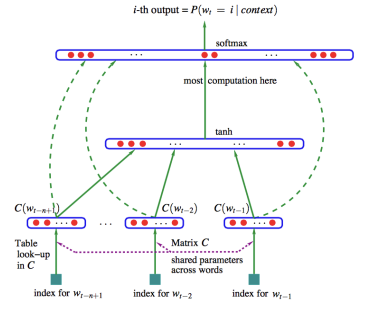
\includegraphics[width=0.62\linewidth,height=\textheight,keepaspectratio,alt={A window-based neural language model}]{assets/img/posts/language-models-and-rnns/window-neural-language-model.png}
\caption{A window-based neural language model}
\end{figure}

The model above can be written as

\[
\hat{y}
=\operatorname{softmax}\left(
W^{(2)}\tanh\left(W^{(1)}x+b^{(1)}\right)
+W^{(3)}x+b^{(3)}
\right).
\]

Here, \(W^{(1)}\) acts on the word vectors, \(W^{(2)}\) acts on the
hidden layer, and \(W^{(3)}\) acts directly on the word vectors.

\begin{figure}
\centering
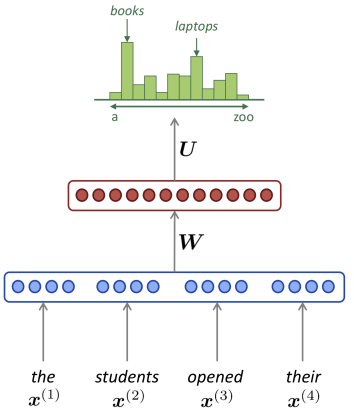
\includegraphics[width=0.48\linewidth,height=\textheight,keepaspectratio,alt={A simplified neural language model}]{assets/img/posts/language-models-and-rnns/simplified-neural-language-model.png}
\caption{A simplified neural language model}
\end{figure}

In the simplified model above, the vectors of multiple input words are
concatenated:

\[
e=[e^{(1)};e^{(2)};e^{(3)};e^{(4)}].
\]

The concatenated vector then passes through a hidden layer,
\(h=f(We+b_1)\), and finally produces the output distribution
\(\hat{y}=\operatorname{softmax}(Uh+b_2)\).

\section{Recurrent Neural Networks
(RNNs)}\label{recurrent-neural-networks-rnns}

Unlike traditional language models, which use only a fixed-length
history window, a recurrent neural network can condition its predictions
on information carried by all previous words. The following diagram
shows the structure of an RNN.

\begin{figure}
\centering
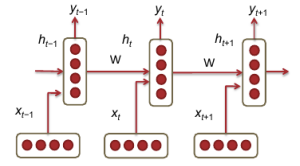
\includegraphics[width=0.62\linewidth,height=\textheight,keepaspectratio,alt={The structure of a recurrent neural network}]{assets/img/posts/language-models-and-rnns/rnn-structure.png}
\caption{The structure of a recurrent neural network}
\end{figure}

Each vertical rectangle represents the hidden layer at time step \(t\).
A hidden layer contains several neurons, each of which first applies a
linear matrix operation and then a nonlinear function. At each time
step, the hidden layer receives two inputs: the previous hidden state
\(h_{t-1}\) and the current input \(x_t\). The former is multiplied by
the weight matrix \(W^{(hh)}\), while the latter is multiplied by
\(W^{(hx)}\). Together, they produce the hidden representation \(h_t\).
The hidden state is then multiplied by \(W^{(S)}\) and passed through a
softmax over the vocabulary to produce the predicted distribution
\(\hat{y}_t\) for the next word:

\[
\begin{aligned}
h_t
&=\sigma\left(W^{(hh)}h_{t-1}+W^{(hx)}x_t\right),\\
\hat{y}_t
&=\operatorname{softmax}\left(W^{(S)}h_t\right).
\end{aligned}
\]

The same \(W^{(hh)}\) and \(W^{(hx)}\) are reused at every time step.
The model therefore has fewer parameters to learn; more importantly, the
number of parameters is independent of the input sequence length,
avoiding the curse of dimensionality.

\subsection{RNN Loss and Perplexity}\label{rnn-loss-and-perplexity}

RNNs commonly use the cross-entropy loss introduced in the previous
notes. At time step \(t\), summing over the entire vocabulary gives

\[
\mathcal{J}^{(t)}(\theta)
=-\sum_{j=1}^{\lvert V\rvert}y_{t,j}\log\hat{y}_{t,j}.
\]

For a corpus of size \(T\), the overall cross-entropy is

\[
J
=\frac{1}{T}\sum_{t=1}^{T}\mathcal{J}^{(t)}(\theta)
=-\frac{1}{T}\sum_{t=1}^{T}\sum_{j=1}^{\lvert V\rvert}
y_{t,j}\log\hat{y}_{t,j}.
\]

The following equation defines \textbf{perplexity}. When the logarithm
in the cross-entropy is base \(2\), perplexity is the exponential form
of that cross-entropy:

\[
\operatorname{Perplexity}=2^J.
\]

Lower perplexity means that the model is more confident in its
predictions of the next word and, in general, agrees more closely with
the observed sequence.

\subsection{Limitations of RNNs}\label{limitations-of-rnns}

RNNs are not a universal solution. They have several limitations:

\begin{itemize}
\tightlist
\item
  Computation is slow because it proceeds sequentially and is difficult
  to parallelize.
\item
  In practice, it is difficult to use information from the distant past
  effectively, partly because of vanishing and exploding gradients.
\end{itemize}

\subsection{Vanishing and Exploding
Gradients}\label{vanishing-and-exploding-gradients}

An RNN repeatedly propagates the same weight matrix from one time step
to the next. One of its goals is to carry contextual information across
long temporal distances. However, information from much earlier time
steps may disappear during backpropagation; this is known as the
\textbf{vanishing-gradient problem}. The mathematical reason is
described below.

To compute the total error gradient with respect to the parameter \(W\),
we sum the error gradients from all time steps:

\[
\frac{\partial E}{\partial W}
=\sum_{t=1}^{T}\frac{\partial E_t}{\partial W}.
\]

Applying the chain rule to the gradient at a single time step gives

\[
\frac{\partial E_t}{\partial W}
=\sum_{k=1}^{t}
\frac{\partial E_t}{\partial y_t}
\frac{\partial y_t}{\partial h_t}
\frac{\partial h_t}{\partial h_k}
\frac{\partial h_k}{\partial W}.
\]

Here, \(\frac{\partial h_t}{\partial h_k}\) is the gradient of the
hidden state at time \(t\) with respect to the hidden state at time
\(k\). By the chain rule,

\[
\frac{\partial h_t}{\partial h_k}
=\prod_{j=k+1}^{t}\frac{\partial h_j}{\partial h_{j-1}}
=\prod_{j=k+1}^{t}W^\top
\operatorname{diag}\left[f'(h_{j-1})\right].
\]

The total gradient is therefore

\[
\frac{\partial E}{\partial W}
=\sum_{t=1}^{T}\sum_{k=1}^{t}
\frac{\partial E_t}{\partial y_t}
\frac{\partial y_t}{\partial h_t}
\left(
\prod_{j=k+1}^{t}\frac{\partial h_j}{\partial h_{j-1}}
\right)
\frac{\partial h_k}{\partial W}.
\]

Suppose that

\[
\left\lVert W^\top\right\rVert\le\beta_W,
\qquad
\left\lVert\operatorname{diag}\left[f'(h_{j-1})\right]\right\rVert
\le\beta_h.
\]

Then

\[
\left\lVert\frac{\partial h_j}{\partial h_{j-1}}\right\rVert
\le\beta_W\beta_h,
\qquad
\left\lVert\frac{\partial h_t}{\partial h_k}\right\rVert
\le(\beta_W\beta_h)^{t-k}.
\]

Therefore:

\begin{itemize}
\tightlist
\item
  If \(\beta_W\beta_h<1\), the gradient decays exponentially over time,
  producing a \textbf{vanishing gradient}.
\item
  If \(\beta_W\beta_h>1\), the gradient may grow exponentially,
  producing an \textbf{exploding gradient}.
\end{itemize}

\subsection{Remedies for Exploding and Vanishing
Gradients}\label{remedies-for-exploding-and-vanishing-gradients}

\textbf{Exploding gradients}

When the gradient norm exceeds a threshold, we scale the gradient to a
fixed range:

\[
\hat{g}\leftarrow\frac{\partial E}{\partial W},
\qquad
\left\lVert\hat{g}\right\rVert\ge\operatorname{threshold}
\Rightarrow
\hat{g}\leftarrow
\frac{\operatorname{threshold}}{\left\lVert\hat{g}\right\rVert}\hat{g}.
\]

This method is called \textbf{gradient clipping}. It preserves the
direction of the gradient while limiting its magnitude, preventing
excessively large parameter updates.

\textbf{Vanishing gradients}

Common approaches include:

\begin{itemize}
\tightlist
\item
  Initialize \(W^{(hh)}\) as the identity matrix rather than randomly.
\item
  Use ReLU instead of sigmoid. The derivative of ReLU is either \(0\) or
  \(1\); where it is \(1\), the gradient does not continuously decay as
  it propagates backward through time.
\end{itemize}

\subsection{Deep Bidirectional RNNs}\label{deep-bidirectional-rnns}

So far, we have focused on RNNs that predict the next word from previous
words. By allowing another RNN to read the corpus in reverse, we can
also use information from future words. A standard RNN uses only past
information, whereas a bidirectional RNN maintains two hidden states:

\begin{itemize}
\tightlist
\item
  \(\overrightarrow{h_t}\) propagates from left to right and encodes
  past information.
\item
  \(\overleftarrow{h_t}\) propagates from right to left and encodes
  future information.
\end{itemize}

\[
\begin{aligned}
\overrightarrow{h_t}
&=f\left(
\overrightarrow{W}x_t
+\overrightarrow{V}\overrightarrow{h}_{t-1}
+\overrightarrow{b}
\right),\\
\overleftarrow{h_t}
&=f\left(
\overleftarrow{W}x_t
+\overleftarrow{V}\overleftarrow{h}_{t+1}
+\overleftarrow{b}
\right).
\end{aligned}
\]

\begin{figure}
\centering
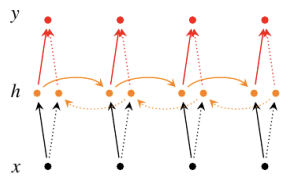
\includegraphics[width=0.62\linewidth,height=\textheight,keepaspectratio,alt={A bidirectional RNN}]{assets/img/posts/language-models-and-rnns/bidirectional-rnn.png}
\caption{A bidirectional RNN}
\end{figure}

The hidden states from the two directions are concatenated to make a
prediction:

\[
\hat{y}_t
=g\left(U[\overrightarrow{h_t};\overleftarrow{h_t}]+c\right).
\]

A bidirectional RNN can use context on both sides of the current
position, but it must maintain two sets of hidden states and parameters.

\textbf{Deep bidirectional RNNs}

RNNs can be stacked into multiple layers. The output of a lower layer
becomes the input to the next layer at the same time step. For layer
\(i\),

\[
\begin{aligned}
\overrightarrow{h_t}^{(i)}
&=f\left(
\overrightarrow{W}^{(i)}h_t^{(i-1)}
+\overrightarrow{V}^{(i)}\overrightarrow{h}_{t-1}^{(i)}
+\overrightarrow{b}^{(i)}
\right),\\
\overleftarrow{h_t}^{(i)}
&=f\left(
\overleftarrow{W}^{(i)}h_t^{(i-1)}
+\overleftarrow{V}^{(i)}\overleftarrow{h}_{t+1}^{(i)}
+\overleftarrow{b}^{(i)}
\right).
\end{aligned}
\]

The two directional hidden states from the highest layer are used for
prediction:

\[
\hat{y}_t
=g\left(U[\overrightarrow{h_t}^{(L)};\overleftarrow{h_t}^{(L)}]+c\right).
\]

\begin{figure}
\centering
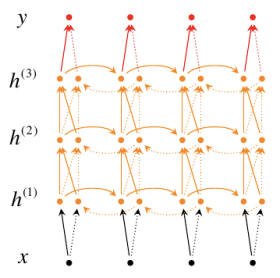
\includegraphics[width=0.55\linewidth,height=\textheight,keepaspectratio,alt={A deep bidirectional RNN}]{assets/img/posts/language-models-and-rnns/deep-bidirectional-rnn.png}
\caption{A deep bidirectional RNN}
\end{figure}

\section{Gated Recurrent Units (GRUs)}\label{gated-recurrent-units-grus}

Beyond these extensions, researchers have found that more complex
activation units can improve RNN performance. So far, we have
transformed \(h_{t-1}\) into \(h_t\) using an affine transformation
followed by an element-wise nonlinearity. A GRU changes this structure
by introducing \textbf{gated activation functions}.

Although an RNN can theoretically capture long-term dependencies, it is
difficult to train one to do so reliably in practice. The GRU is
designed to preserve memory more easily over long periods, making
long-range dependencies easier to capture. It generates the next hidden
state \(h_t\) from \(h_{t-1}\) and \(x_t\) in four steps:

\begin{enumerate}
\def\labelenumi{\arabic{enumi}.}
\item
  \textbf{Update gate:} Determines how much of the previous hidden state
  \(h_{t-1}\) is retained directly in the current state.

  \[
  z_t=\sigma\left(W^{(z)}x_t+U^{(z)}h_{t-1}\right).
  \]

  When \(z_t\approx1\), the unit mainly preserves the old memory. When
  \(z_t\approx0\), it mainly uses the new memory.
\item
  \textbf{Reset gate:} Determines how much past information is used when
  generating the new memory.

  \[
  r_t=\sigma\left(W^{(r)}x_t+U^{(r)}h_{t-1}\right).
  \]

  The smaller \(r_t\) is, the more the unit tends to ignore the previous
  hidden state when generating new memory.
\item
  \textbf{New memory generation:} Combines the current input \(x_t\)
  with past information filtered by the reset gate to produce a
  candidate hidden state.

  \[
  \widetilde{h}_t
  =\tanh\left(r_t\circ Uh_{t-1}+Wx_t\right).
  \]
\item
  \textbf{Hidden state:} Uses the update gate to form a weighted
  combination of the old memory \(h_{t-1}\) and the new memory
  \(\widetilde{h}_t\).

  \[
  h_t
  =(1-z_t)\circ\widetilde{h}_t
  +z_t\circ h_{t-1}.
  \]
\end{enumerate}

\begin{figure}
\centering
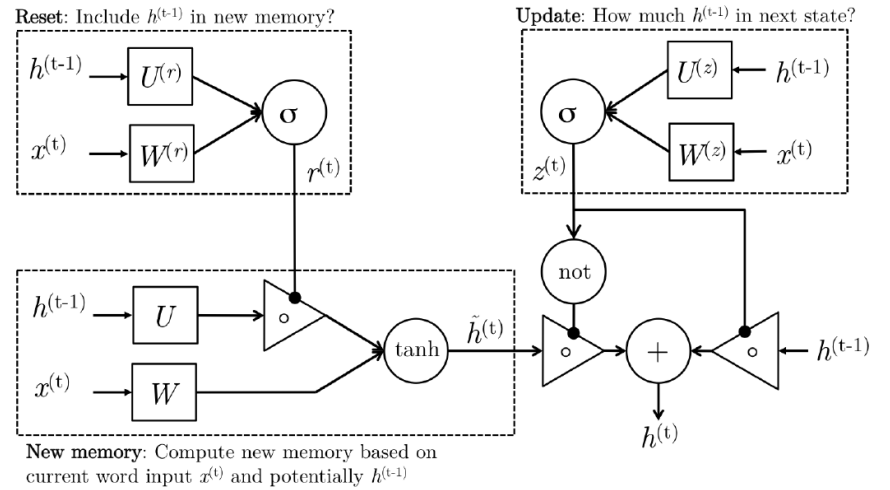
\includegraphics[width=0.9\linewidth,height=\textheight,keepaspectratio,alt={The gated structure of a GRU}]{assets/img/posts/language-models-and-rnns/gru.png}
\caption{The gated structure of a GRU}
\end{figure}

\section{Long Short-Term Memory Networks
(LSTMs)}\label{long-short-term-memory-networks-lstms}

An LSTM controls information flow with an \textbf{input gate}, a
\textbf{forget gate}, and an \textbf{output gate}. It also maintains a
memory cell \(c_t\) that stores long-term information. The LSTM can be
understood in the following stages:

\begin{enumerate}
\def\labelenumi{\arabic{enumi}.}
\item
  \textbf{New memory generation:} Generates candidate memory from the
  current input \(x_t\) and the previous hidden state \(h_{t-1}\).

  \[
  \widetilde{c}_t
  =\tanh\left(W^{(c)}x_t+U^{(c)}h_{t-1}\right).
  \]
\item
  \textbf{Input gate:} Determines how much of the candidate memory
  \(\widetilde{c}_t\) is written to the current memory.

  \[
  i_t=\sigma\left(W^{(i)}x_t+U^{(i)}h_{t-1}\right).
  \]
\item
  \textbf{Forget gate:} Determines how much information from the
  previous memory \(c_{t-1}\) is retained.

  \[
  f_t=\sigma\left(W^{(f)}x_t+U^{(f)}h_{t-1}\right).
  \]
\item
  \textbf{Final memory generation:} Combines the retained old memory
  with the newly written memory to produce the current memory \(c_t\).

  \[
  c_t
  =f_t\circ c_{t-1}
  +i_t\circ\widetilde{c}_t.
  \]
\item
  \textbf{Output gate and hidden state:} The output gate determines how
  much of the memory \(c_t\) is exposed through the hidden state
  \(h_t\).

  \[
  o_t=\sigma\left(W^{(o)}x_t+U^{(o)}h_{t-1}\right),
  \qquad
  h_t=o_t\circ\tanh(c_t).
  \]
\end{enumerate}

In summary:

\begin{itemize}
\tightlist
\item
  \(i_t\) controls \textbf{how much new information is written}.
\item
  \(f_t\) controls \textbf{how much old information is retained}.
\item
  \(o_t\) controls \textbf{how much of the current memory is exposed}.
\item
  \(c_t\) is the long-term memory.
\item
  \(h_t\) is the hidden state exposed at the current time step.
\end{itemize}

\begin{figure}
\centering
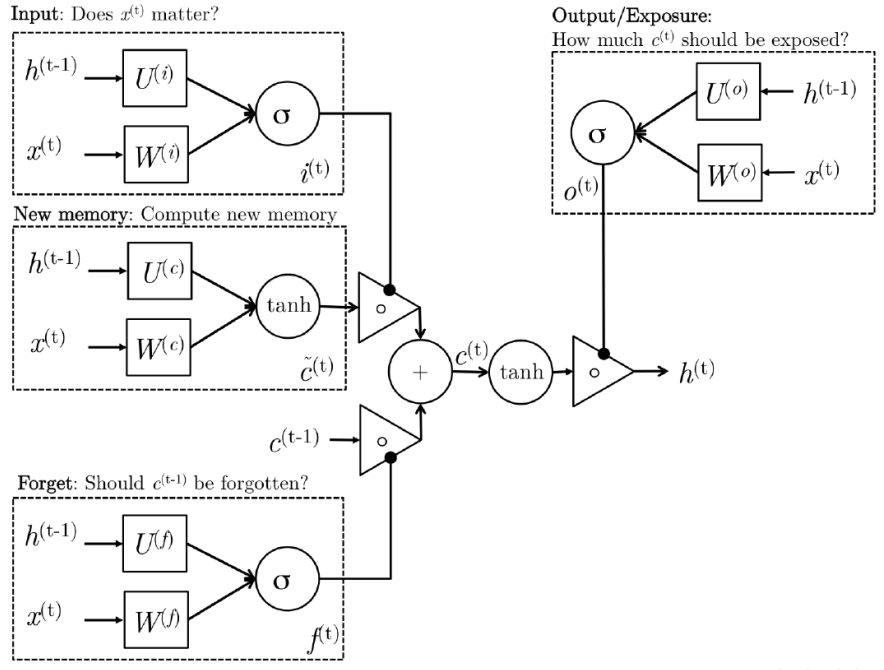
\includegraphics[width=0.9\linewidth,height=\textheight,keepaspectratio,alt={The gated structure of an LSTM}]{assets/img/posts/language-models-and-rnns/lstm.png}
\caption{The gated structure of an LSTM}
\end{figure}

\end{document}
